\textbf{Cet exercice comporte quatre questions indépendantes.}

Toutes les questions doivent être traitées.

\subsection*{Question 1}

On considère ci-dessous la courbe représentative $\mathcal{C}$ d'une fonction $f$ définie sur
l'intervalle [2 ; 8].

\begin{center}
%%%Début PS Tricks
%\psset{xunit=0.78cm,yunit=0.78cm,labelFontSize=\scriptstyle,showorigin=false}
%	\begin{pspicture}(-1.1,-1.5)(10.5,9.5)
%		\multido{\n=-1+1}{12}{\psline[linewidth=0.75pt,linecolor=lightgray](\n,-1.1)(\n,9)}
%		\multido{\n=-1+1}{11}{\psline[linewidth=0.75pt,linecolor=lightgray](-1.1,\n)(10.3,\n)}
%		\uput[dl](0,0){\footnotesize 0}\uput[u](7.5,2.35){$\mathcal{C}$}
%		\psaxes[linewidth=0.95pt]{->}(0,0)(-1.2,-1.5)(10.5,9.35)
%		\pscurve[linewidth=1.5pt,linecolor=blue](2,5)(3,4.91)(4,4.6)(5,4.1)(6,3.4)(7,2.5)(8,1.5)
%	\end{pspicture}
%%%Fin PS tricks
%Début tikz
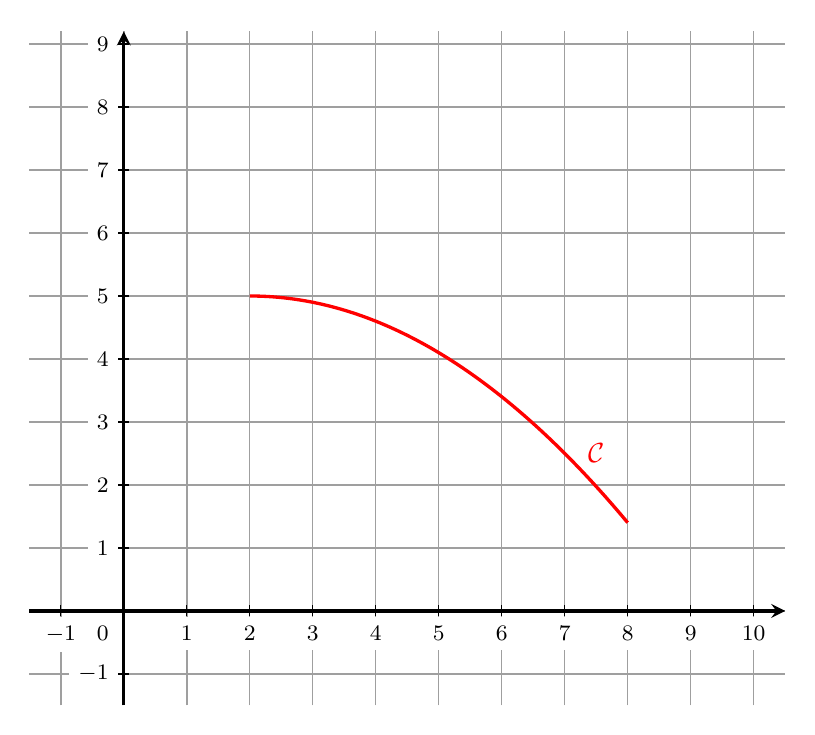
\begin{tikzpicture}[x=8mm,y=8mm,>=stealth]

	\draw [color = gray!75, line width = 0.5pt, xstep=1, ystep = 1] (-1.5,-1.5) grid (10.5,9.2);
	\foreach \x in {-1,1,2,...,10}
	\draw[shift={(\x,0)},color=black] (0pt,2pt) -- (0pt,-2pt) node[below, fill = white] {\footnotesize $\np{\x}$};
	\foreach \y in {-1,1,2,...,9}
	\draw[shift={(0,\y)},color=black] (2pt,0pt) -- (-2pt,0pt) node[left, fill = white] {\footnotesize $\np{\y}$};
	\draw [->, line width = 1.2pt] (-1.5,0)--(10.5,0);
	\draw [->, line width = 1.2pt] (0,-1.5)--(0,9.2);
	\draw[color=black] (-2pt,-2pt) node[below left] {\footnotesize 0};
	\draw[line width=1.2pt,color=red,smooth,samples=100,domain= 2:8 ] plot(\x,{5-(\x-2)*(\x-2)/10} );
	\node[red] at (7.5,2.5) {$\mathcal{C}$};
\end{tikzpicture}
%Fin tikz
\end{center}

Par lecture graphique, donner la valeur de $f(2)$.

\subsection*{Question 2}

Soit $g$ la fonction définie sur l'intervalle $]0 ; +\infty[$ par $g(x)=x^2 + 2x + \ln(x)$.

On admet que la fonction $g$ est dérivable sur l'intervalle $]0 ; +\infty[$ et on note $g'$ sa
fonction dérivée.

Calculer $g'(x)$.


\subsection*{Question 3}
On considère l'équation différentielle (E) :
\[  y'=-2 y.   \]
Déterminer l'ensemble des solutions de (E).


\subsection*{Question 4}


Soit $h$ une fonction définie sur l'intervalle [2 ; 5].

On admet que $\displaystyle \int_{2}^{5} h(x) \d(x)=6$


Calculer la valeur moyenne de $h$ sur l'intervalle [2 ; 5].
